%% INIZIO CONTENUTO TESI
%% TODO: Create a section where to explain the system's teminology.
%% * Any term inside the section will be start with the capital letter
%% * (es. Archived, Annotation, etc.)
\mainmatter
\chapter{Introduzione}
\label{cap:introduzione}

\section{L'azienda}
Lo stage formativo è stato svolto presso l'azienda Wonderflow, fondata nel 2014
ad Amsterdam. Wonderflow si colloca nel mercato \gls{B2B}
offrendo alle aziende una \gls{dashboard}, denominata \textbf{Wonderboard}, in
cui le compagnie registrano i loro prodotti e ottengono una serie di
statistiche sull'andamento del gradimento e commenti degli utenti utili per
poter migliorare i propri articoli.

\begin{figure}[htbp]
\begin{center}

\includegraphics[height=2cm]{wonderflow-logo}
\caption{Logo Wonderflow}
\end{center}
\end{figure}

\subsection{I ruoli}
La Wonderflow è suddivisa in tre gruppi: analisti, sviluppatori e venditori.

E' importante comprendere il ruolo dell'\textbf{analista} e dello
\textbf{sviluppatore} all'interno dell'azienda ed il loro modo di lavorare in
quanto l'intera esperienza di stage gira attorno a queste due figure.

\subsubsection{Analisti}
La raccolta delle informazioni sui prodotti è compiuta dal team di
\textbf{analisti} attraverso l'analisi delle recensioni di un prodotto, prese
da vari siti web di vendita, al fine di individuare frasi chiavi in cui
emerge un \textbf{sentimento}, denominate \textbf{annotazioni}.
\newline

L'analisi delle recensioni avviene attraverso un \textbf{editor} interno dove
viene visualizzato il testo di ciascuna recensione in modo che l'analista
possa, in modo semplice ed intuitivo, evidenziare le annotazioni all'interno di
un testo, associarvi un sentimento e salvarle nell'archivio della Wonderflow.
\newline

Vi sono altri aspetti nella creazione delle annotazioni ma verranno trattati
nel capitolo dedicato all'esposizione del progetto in modo da avere un contesto
adeguato per comprendergli meglio. Per quanto riguarda la procedura di
elaborazione delle annotazioni per ottenere i dati visualizzati dalla
Wonderboard, questa non verrà trattata in quanto fuori dall'argomento dello
stage.

\subsubsection{Sviluppatori}
Il gruppo \textbf{sviluppatori} realizza gli strumenti software usati
internamente all'azienda e scarica le recensioni per poi fornirle agli analisti.
\newline

Data il loro ridotto numero, le conoscenze di ognuno non erano circoscritte al
proprio ruolo ma, per venire incontro alle esigenze dell'azienda, si
espandevano per una buona parte dell'organizzazione, in modo da avere maggior
comprensione sul lavoro da svolgere. Non era inusuale che il programmatore
conoscesse il flusso di lavoro dell'analista o apprendesse tecniche di vendita
o prendesse decisioni sull'impostazione dell'azienda. Tutto ciò aumentava il
senso di appartenenza ed importanza della persona dentro il contesto aziendale.
\newline

Le interazioni tra sviluppatore e analista o venditore avvengono in modo
diretto, non formale e senza passare per un ente supervisore. In questa maniera
la comprensione dei requisiti diventava più veloce; si generava un rapporto tra
i membri dell'azienda più stretto ed un ambiente di lavoro più rilassato.
\newline

L'organizzazione dei compiti assegnati sono auto-organizzate dall'assegnatario.
Lo sviluppatore decide come affrontare un problema, progettare la soluzione ed
implementarla usando le risorse a disposizione. Il motivo è lasciare che nuovi
sviluppatori portino dentro alla compagnia il proprio bagaglio di conoscenze e
che queste vengano subito condivise ed applicate senza ostacoli, in modo da
accumulare idee e metodologie al passo coi tempi.

\section{L'organizzazione}
Da come si può dedurre dalla metodologia di lavoro descritta sopra, la
Wonderflow, come tante altre piccole case produttrici di software, aderisce
al metodo di sviluppo \gls{agile} e usa \gls{scrum}, figura
\ref{fig:scrum_process}, come modello di ciclo di sviluppo.

\begin{figure}[ht]
\begin{center}
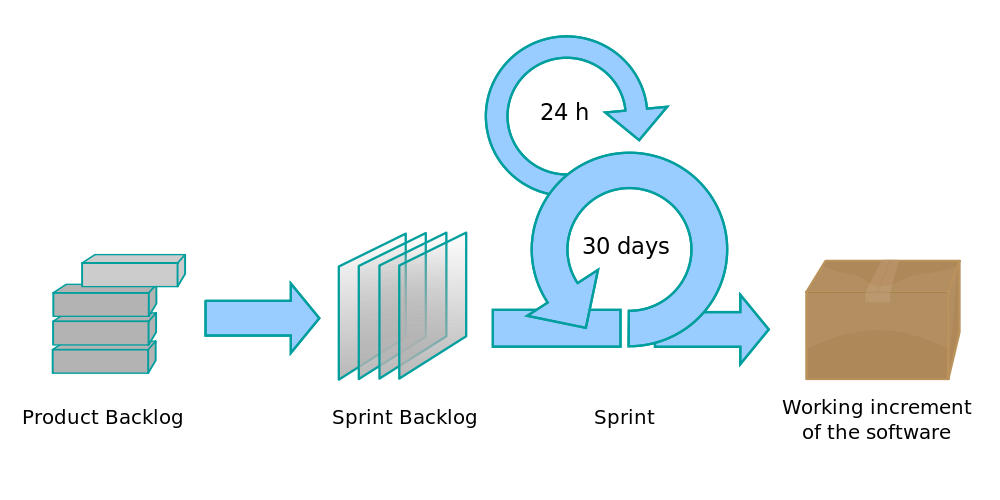
\includegraphics[height=5cm]{scrum_process}
\caption{Rappresentazione modello di sviluppo Scrum}
\label{fig:scrum_process}
\end{center}
\end{figure}

\subsection{Attività giornaliere}
Seguendo \gls{scrum}, ogni giornata lavorativa inizia con lo
\textit{standup meeting}, nel quale attraverso il programma di messaggistica
\textit{Slack} si invia il riassunto delle attività svolte il giorno prima,
quelle che si andranno a compiere il giorno stesso ed eventuali ostacoli che
presumibilmente si incontreranno. Una volta terminato il meeting si inizia con
lo sviluppo fino all'ora fissata per il \textit{daily}, una riunione generale
dove \textbf{ogni} membro della compagnia è chiamato a presentare agli altri il
lavoro svolto durante la giornata, lo stato attuale del lavoro, difficoltà
trovate e i dubbi sorti.

\subsection{Sviluppo}
Il \textit{tutor} aziendale ha organizzato lo stage in \gls{sprint} della
durata di una settimana. Ogni \gls{sprint} corrisponde ad un'aspetto del
progetto, da integrare assieme una volta conclusi. La chiusura dello
\gls{sprint} implica una prima fase di \gls{verifica} per accertare che il
codice prodotto sia conforme agli standard dell'azienda. Nel caso d'esito
positivo il prodotto finale viene rilasciato, altrimenti viene trascritta la
lista dei difetti riscontrati da risolvere, ritornando cosi allo sviluppo. Una
volta apportate le modifiche correttive venivi riapplicata la verifica. Questa
procedura continuava finché il risulto non fosse confacente alle aspettative.
\newline

Gli standard fissati dalla Wonderflow mirano nell'avere il codice il più
comprensibile possibile in modo che futuri sviluppatori siano capaci in poco
tempo a lavorare con esso ed in completa autonomia. Le caratteristiche che si
vanno ad ispezionare sono:
\paragraph{Logica}
E' importante non produrre algoritmi complessi che potrebbero richiedere un
certo quantitativo di tempo per studiarli e comprenderli. Meglio produrre
programmi semplici adattati ad hoc per la situazione.

\paragraph{Nomi}
I nomi per le variabili, funzioni, classi, ecc... devono essere comprensibili
e fornire al lettore un'idea del suo scopo. Inoltre i nomi delle funzioni
devono dare una qualche informazione sui suoi parametri per colmare l'assenza
di documentazione.

\paragraph{Organizzazione}
Dividere il progetto in vari file (uno per classe) e raccoglierli in cartelle
denominate in base all'area tematica toccata aiuta ad orientarsi durante lo
sviluppo, fondamentale soprattutto quando si esegue il \gls{refactoring} del
codice.

\paragraph{Progettazione}
Per garantire un semplice utilizzo dei vari progetti realizzati è importante
soddisfare due fattori: \textbf{dimensioni} e \textbf{semplicismo}.
La prima è tanto più buona quanto è più ridotta. Progetti di piccoli dimensioni
sono facili da gestire, comprendere e risultano maggiormente mantenibili. E'
inoltre possibile poter agilmente cambiare lo sviluppatore che ne fa uso
garantendo l'indipendenza sul personale.

Per quanto riguarda la seconda, vengono apprezzate maggiormente soluzioni di
\textit{design} non elaborate e di facile comprensione, sempre per acconsentire
una rapida comprensione del software anche con scarsa, o addirittura assente,
documentazione. \\

Il principale obiettivo é produrre codice comprensibile. Spesso la
soddisfazione dei requisiti appena descritti non corrisponde ad un risultato
completo e caratteristiche come la resilienza, robustezza o estendibilità
potevano essere assenti, almeno nelle prive versioni. Il tempo dedicato
alla progettazione iniziale veniva ridotto in favore di rilasci più frequenti,
con l'uso continuo del \gls{refactoring}.

E' importante sottolineare questi aspetti in quanto si riflettono
inevitabilmente sulle varie scelte compiute nello svolgere le varie mansioni.
